% ============================================================
% M3 S2 导学件·波1 片件 —— 课时15 2.7.1 抛物线的标准方程（母版照抄制·臂4）
% 生成：M3 成卷轮 S2 波1 臂4｜2026-09-14｜编译 cwd＝本目录（中文路径禁 \input 绝对路径）
%   xelatex main-true.tex ×2 → 含详解印本；xelatex main-false.tex ×2 → 纯题版（单源双本）
% 输入链（全只读）：题面库 课时15-2.7.1抛物线方程.md（题面逐字装配）＋ -答案侧.md（值逐字回嵌）
%   ＋ 定稿/批D-课时15-2.7.1抛物线方程.md（详解回嵌源＝§七 补产 31 块【详解】＋件末「导学 G5 补产」5 键）；
%   toolchain＝qp-m3.sty（钉后版 md5 7c3930362be8a0a2bdf21bbf8ac16573，本地挂载副本，破损即停）。
% 母版体例：详见 成卷/导学件/课时01-坐标法/母版体例说明.md（骨架/宏用法/门谱/坑）。
% 键账：件内 ansblock 键集 ≡ 题面库片键集 ≡ manifest 键序（36 键，零缺漏零多余）；
%   预习位零键零答案；印面号 1—36＝探究 1—31＋课堂评价 32—36，键↔号映射见 值台账-课时15.json。
% 多选门：本片多选 3 道（拓15-03/04/06，印面 26/27/29）≤4 合规，成卷未增；
%   印面带 \duoxuan\hspace{0.6em} 标记＋\lxopt 每选项一行。
% 图注回补：印23（15-16 隧道）、印24（拓15-01 桥拱）题面末随注回补源图尺寸（批D 勘误/转置口径承入）。
% 印面符号口径：源件纯文本扁平记号按数学语义恢复印刷形——向量 PQ=NF 印 \overrightarrow 形、
%   全等≌ 印 \cong、推出向箭头改「得/即」文读；值行 \ansitem 第二参不涉此口径（字节级照录）。
% 括线判据（承重墙禁放宽）：估高＞8 行（chars/23 栏宽口径）→ 括线模，逐键读数入值台账；
%   其余灰底。本片括线键以门谱首轮读数为准（见值台账括线判模口径）。
% 门谱读数：见 过程件 工作区/_tmpM3S2波1臂4_0914/（编译 log、门谱输出、台账）。
% ============================================================
\documentclass[fontset=none]{ctexart}
\usepackage{qp-m3}
% —— 印面逐字符号路由补钉（探针实证 0914：书宋缺 U+2212，▱ 诸字库皆缺→NSC 子块；
%     禁改 sty 本体保 md5；无 ▱/− 用件的片可整块照抄，零副作用） ——
\xeCJKDeclareCharClass{Default}{"2212}%
\setCJKfamilyfont{nscblk}[Path=C:/提示词/工作区/字替对照-0909/variantF/fonts/,BoldFont=NSC-w600.ttf]{NSC-w500.ttf}%
\xeCJKDeclareSubCJKBlock{nscblk}{"25B1}%
\newcommand{\pxparallelogram}{{\CJKfamily{nscblk}▱}}%
% —— 断行微调（纯题档/详解档三零门：CJK 胶收缩；Underfull 治理读数见过程件） ——
\xeCJKsetup{CJKglue={\hskip 0.10em plus 0.08em minus 0.05em}}%
% —— 页脚件名（qp-headfoot 复用入口） ——
\renewcommand{\qpzhangming}{第二章\quad 平面解析几何}%
\renewcommand{\qpjianming}{导学件}%

\begin{document}
%装配轮S6三本跨本连续页码（G7方案B）setcounter 注入位
\setcounter{page}{105}

\zhangtitle{第二章\quad 平面解析几何}
\jietitle{2.7.1 抛物线的标准方程}
\mubiaoline
\mubiaomu{1}{掌握抛物线的定义（定点不在定直线上的等距点集），理解焦点、准线、焦准距的含义，会依据定义识别轨迹并检验定义前提；}
\mubiaomu{2}{掌握抛物线四种标准方程与开口方向、焦点坐标、准线方程的对应关系，会依焦点、准线、焦准距或过定点条件求标准方程，能处理开口待定的双解问题；}
\mubiaomu{3}{会用焦半径与定义互化求距离、点坐标与最值，能建立抛物线模型解决拱桥、隧道、路灯等实际应用问题，体会待定系数、分类讨论与转化思想.}

\vspace{1.7mm}
\begin{multicols}{2}
\emergencystretch=1em

% ============================================================
% 课前预习（知识点导学填空；零键零答案——\kongbai 空线＋\zhentib 判断题面形，
% 两档等形不泄答）
% ============================================================
\huaxing{课}{前}{预}{习}{知识导学\quad 素养初识}

\zsd{一}{抛物线的定义与四种标准方程}

\tiaomu{1}{平面内与定点\(F\)和定直线\(l\)（\(l\)不经过\(F\)）的距离相等的点的轨迹叫做抛物线，定点\(F\)叫做抛物线的\kongbai{}，定直线\(l\)叫做抛物线的\kongbai{}；焦点到准线的距离为\(p\)（焦准距）．\zhuzhu{定义的前提是定点不在定直线上；若定点在定直线上，轨迹是过定点且垂直于定直线的直线，不是抛物线.}}

\tiaomu{2}{四种标准方程与几何量对应：\(y^{2}=2px\)（\(p>0\)）开口向右，焦点为\kongbai{}，准线方程为\kongbai{}；\(y^{2}=-2px\)开口向左，\(x^{2}=2py\)开口向上，\(x^{2}=-2py\)开口向下．\zhuzhu{对称轴由一次项变量确定（一次项为\(x\)则轴为\(x\)轴），开口方向由系数符号确定（系数为负即向负方向开口）.}}

\zsd{二}{依条件求标准方程}

\tiaomu{1}{定向求方程：给焦点或准线位置先定开口方向，再设标准式，由焦准距、焦点坐标或准线方程定\(p\)；开口未指定时，\kongbai{}种标准方程并立．\zhuzhu{只过一定点而未定向时，按可能经过该点的开口方向分类补全（如点在第四象限考虑开口向右、向下两类），防止漏解.}}

\tiaomu{2}{系数直读：\(y^{2}=mx\)（\(m\neq 0\)）中\(2p=\)\kongbai{}，焦点横标为\kongbai{}；由准线方程反求\(p\)时，注意开口方向与准线位置一致．\zhuzhu{含参开壳如\(y^{2}=4ax\)：\(a>0\)开口向右，\(a<0\)开口向左，焦点\((a,0)\)形式不变；先化标准形再读几何量.}}

\zsd{三}{焦半径与实际应用}

\tiaomu{1}{焦半径：抛物线上点\(P\)到焦点的距离等于它到准线的距离，如\(y^{2}=2px\)上\(|PF|=\)\kongbai{}；据此可在距离、点坐标、最值之间互化．\zhuzhu{焦半径坐标式按点所在象限去绝对值；到焦点距离的最小值在顶点处取得，为\(p/2\)，与“恒大于”类开区间条件联用.}}

\tiaomu{2}{实际应用：拱桥、隧道、路灯等轮廓问题，常以顶点为原点、对称轴为坐标轴建系，设标准方程后代已知点求\(p\)，最后回到实际量作答．\zhuzhu{印面无图的题按图注尺寸立式；应用题结论须带单位并回应题问（能否通过、位置如何等）；立体几何背景中的轨迹判定回到定义与圆锥曲线截线语义.}}

\zhenhead{判断正误(正确的打\gou{},错误的打\cha{})}

\zhentib{(1)}{平面内到定点\(A\)与到定直线\(l\)的距离相等的点的轨迹一定是抛物线．}

\zhentib{(2)}{抛物线\(x^{2}=2py\)（\(p>0\)）的焦点坐标为\((0,p/2)\)，准线方程为\(y=-p/2\)．}

\liubai[9mm]{此处书写}

% ============================================================
% 课中探究（考点探究〔例+变式〕＝练槽 31 键；题后紧跟答案＝ansblock 内嵌，
% 值照答案侧逐字，详解承批D §七【详解】/「导学 G5 补产」回嵌＋印面清洗）
% ============================================================
\huaxing{课}{中}{探}{究}{考点探究\quad 素养小结}

% ---------- 探究点一 抛物线的定义与轨迹判定（印面 1—5） ----------
\tjdnr{一}{抛物线的定义与轨迹判定}{例\textbf{1}}{简单(知识点一)}{【微思考】在抛物线定义中，若去掉条件“\(l\)不经过点\(F\)”，点的轨迹还是抛物线吗？}
\xiexwei{7mm}

{\ansblockgrayfalse
\begin{ansblock}[2章-练-课时15-01]
% ans:2章-练-课时15-01
\ansitem{1}{不是。当定点 F 在直线 l 上时，动点轨迹是与 l 垂直的直线（过 F）。}
\ansnote{详解}{取\(l\)为\(x\)轴、\(F\)为原点．动点\(P(x,y)\)到\(F\)的距离为\(\sqrt{x^{2}+y^{2}}\)，到\(l\)的距离为\(|y|\)．\par\noindent “到\(F\)与到\(l\)距离相等”：\(\sqrt{x^{2}+y^{2}}=|y|\)，平方得\(x^{2}+y^{2}=y^{2}\)，即\(x=0\)．轨迹为整条\(y\)轴：过\(F\)且垂直于\(l\)的直线，不是抛物线（\(p=0\)时抛物线无意义）．验算：点\((0,5)\)到\(F\)距离5、到\(x\)轴距离5，相等合．}
\end{ansblock}}

\liB{变式\textbf{2}}{简单(知识点一)}{}{与点\(F(0,-3)\)和直线\(y-3=0\)的距离相等的点的轨迹方程是\kongbai{}．}
\xiexwei{7mm}

\begin{ansblock}[2章-练-课时15-03]
% ans:2章-练-课时15-03
\ansitem{2}{x²=−12y}
\ansnote{详解}{\(F(0,-3)\)不在直线\(y=3\)上，由定义轨迹为抛物线：焦点\(F(0,-3)\)，准线\(y=3\)．开口向下，设\(x^{2}=-2py\)（\(p>0\)）：\(p/2=3\)，\(p=6\)，方程\(x^{2}=-12y\)．验算：顶点\((0,0)\)到\(F\)距3、到准线距3合．}
\end{ansblock}

\tjdnr{一}{抛物线的定义与轨迹判定}{例\textbf{3}}{简单(知识点一)}{已知实数\(x\)，\(y\)满足\(\sqrt{x^{2}+(y-p/2)^{2}}=|y+p/2|\)，其中常数\(p>0\)，则动点\(P(x,y)\)的轨迹是\nobreak(\kongwei)}

\bindopt {\fontsize{10.5pt}{\qpTJgLeadLiti}\selectfont \makebox[\dimexpr0.5\linewidth-1em\relax][l]{A．射线}\makebox[\dimexpr0.5\linewidth-1em\relax][l]{B．直线}\par}
\bindopt {\fontsize{10.5pt}{\qpTJgLeadLiti}\selectfont \makebox[\dimexpr0.5\linewidth-1em\relax][l]{C．抛物线}\makebox[\dimexpr0.5\linewidth-1em\relax][l]{D．椭圆}\par}

\begin{ansblock}[2章-练-课时15-05]
% ans:2章-练-课时15-05
\ansitem{3}{C}
\ansnote{详解}{左端为\(P(x,y)\)到定点\(F(0,p/2)\)的距离；右端\(|y+p/2|\)为\(P\)到定直线\(l\)：\(y=-p/2\)的距离．\(F(0,p/2)\)不在\(l\)上（\(p>0\)），由抛物线定义，轨迹为抛物线，故选C．}
\end{ansblock}

\liB{变式\textbf{4}}{中档(知识点一)}{}{已知点\(M\)到点\(F(4,0)\)的距离比它到直线\(l\)：\(x+6=0\)的距离小2，求点\(M\)的轨迹方程．}
\xiexwei{7mm}

{\ansblockgrayfalse
\begin{ansblock}[2章-练-课时15-14]
% ans:2章-练-课时15-14
\ansitem{4}{y²=16x。}
\ansnote{详解}{设\(M(x,y)\)．“\(|MF|\)比到\(l\)的距离小2”即\(|x+6|-|MF|=2\)．当\(x\geqslant -6\)时：\(x+6-\sqrt{(x-4)^{2}+y^{2}}=2\)，即\(\sqrt{(x-4)^{2}+y^{2}}=x+4\)（隐含\(x\geqslant -4\)，自然满足），平方得\((x-4)^{2}+y^{2}=(x+4)^{2}\)，化简为\(y^{2}=16x\)（此时\(x\geqslant 0\geqslant -4\)，与所设一致）；\par\noindent 当\(x<-6\)时：\(-x-6-\sqrt{(x-4)^{2}+y^{2}}=2\)，即\(\sqrt{(x-4)^{2}+y^{2}}=-x-4\)，平方同样得\(y^{2}=16x\)，但该抛物线上\(x\geqslant 0\)，与\(x<-6\)矛盾，此段无轨迹．故轨迹方程\(y^{2}=16x\)（顶点在原点、开口向右的抛物线，焦点\(F(4,0)\)、准线\(x=-4\)）．验算：\(y^{2}=16x\)上任一点\(|MF|=x+4\)，到直线\(x=-6\)的距离为\(x+6\)，差恰为2合．\par\noindent 辨析：本题须防“大2”误读——若误作“\(|MF|\)比到直线\(x=-6\)的距离大2”，则\(|MF|=|x+8|\)，平方化简为\(y^{2}=24(x+2)\)，为平移型抛物线（顶点\((-2,0)\)），与标准形不符；按原题“小2”，平移准线得\(|MF|\)等于到直线\(x=-4\)的距离，才落到标准抛物线\(y^{2}=16x\)．}
\end{ansblock}}

\tjdnr{一}{抛物线的定义与轨迹判定}{例\textbf{5}}{简单(知识点一)}{若抛物线\(y^{2}=2px\)（\(p>0\)）上任意一点到焦点的距离恒大于1，则\(p\)的取值范围是\nobreak(\kongwei)}

\bindopt {\fontsize{10.5pt}{\qpTJgLeadLiti}\selectfont \makebox[\dimexpr0.5\linewidth-1em\relax][l]{A．\(p<1\)}\makebox[\dimexpr0.5\linewidth-1em\relax][l]{B．\(p>1\)}\par}
\bindopt {\fontsize{10.5pt}{\qpTJgLeadLiti}\selectfont \makebox[\dimexpr0.5\linewidth-1em\relax][l]{C．\(p<2\)}\makebox[\dimexpr0.5\linewidth-1em\relax][l]{D．\(p>2\)}\par}

\begin{ansblock}[2章-拓-课时15-15]
% ans:2章-拓-课时15-15
\ansitem{5}{D}
\ansnote{详解}{由定义，抛物线上点到焦点的距离等于它到准线\(x=-p/2\)的距离，其最小值在顶点处取得，为\(p/2\)．恒大于\(1\Leftrightarrow p/2>1\Leftrightarrow p>2\)，故选D．验算：\(p=2\)时顶点到焦点距离\(=1\)，不满足“恒大于”，开区间正确合．}
\end{ansblock}

\xiaojie{①识别：给“到定点与定直线距离相等（或不等）”式条件判轨迹、追问定义前提被破坏后轨迹形态的题，判归本题型；第一步核“定点是否在定直线上”.}
\bindp {\kaishu ②操作：定点不在定直线上，轨迹为抛物线；定点在定直线上，轨迹为过定点且垂直于定直线的直线；“距离之和/差为常数”型按常数与已知量比较分段定轨.}
\bindp {\kaishu ③收束：轨迹题写方程须连同坐标范围；退化情形（直线、线段、无轨迹）逐一交代；以“恒大于/恒小于”给出的条件注意开闭区间.}

% ---------- 探究点二 标准方程的求法（印面 6—17） ----------
\liB{变式\textbf{6}}{简单(知识点二)}{}{焦点到准线的距离为\(3/2\)的抛物线的标准方程为\kongbai{}．}
\xiexwei{7mm}

\begin{ansblock}[2章-练-课时15-02]
% ans:2章-练-课时15-02
\ansitem{6}{y²=3x 或 y²=−3x 或 x²=3y 或 x²=−3y。}
\ansnote{详解}{焦准距即\(p\)：\(p=3/2\)，\(2p=3\)．开口未指定，四种标准方程并立：\(y^{2}=3x\)、\(y^{2}=-3x\)、\(x^{2}=3y\)、\(x^{2}=-3y\)．}
\end{ansblock}

\tjdnr{二}{标准方程的求法}{例\textbf{7}}{简单(知识点二)}{分别根据下列条件，写出抛物线的标准方程：(1)焦点是\(F(2,0)\)；(2)准线方程是\(x=-3/2\)．}
\xiexwei{12mm}

\begin{ansblock}[2章-练-课时15-07]
% ans:2章-练-课时15-07
\ansitem{7}{(1) y²=8x；(2) y²=6x。}
\ansnote{详解}{(1)焦点\((2,0)\)在\(x\)正半轴：\(p/2=2\)，\(p=4\)，\(2p=8\)，方程\(y^{2}=8x\)．(2)准线\(x=-3/2\)得焦点在\(x\)正半轴：\(p/2=3/2\)，\(p=3\)，\(2p=6\)，方程\(y^{2}=6x\)．验算：(1)准线\(x=-2\)合；(2)焦点\((3/2,0)\)合．}
\end{ansblock}

\liB{变式\textbf{8}}{简单(知识点二)}{}{写出抛物线\(y^{2}=4ax\)的焦点坐标．}
\xiexwei{7mm}

\begin{ansblock}[2章-拓-课时15-07]
% ans:2章-拓-课时15-07
\ansitem{8}{(a,0)（a≠0）。}
\ansnote{详解}{按标准形\(y^{2}=2px\)对照：\(2p=4a\)，\(p=2a\)，焦点\((p/2,0)=(a,0)\)．\(a>0\)时开口向右，焦点\((a,0)\)；\(a<0\)时开口向左，焦点仍为\((a,0)\)（即\(x\)轴负半轴上）．故焦点\((a,0)\)（\(a\neq 0\)）．验算：\(a=-1\)时\(y^{2}=-4x\)，焦点\((-1,0)\)合．}
\end{ansblock}

\tjdnr{二}{标准方程的求法}{例\textbf{9}}{简单(知识点二)}{写出下列抛物线的焦点坐标和准线方程：(1)\(y=2x^{2}\)；(2)\(y=ax^{2}\)（\(a\neq 0\)）．}
\xiexwei{12mm}

{\ansblockgrayfalse
\begin{ansblock}[2章-拓-课时15-08]
% ans:2章-拓-课时15-08
\ansitem{9}{(1) 焦点 (0,1/8)，准线 y=−1/8；(2) 焦点 (0,1/(4a))，准线 y=−1/(4a)（a≠0）。}
\ansnote{详解}{(1)\(y=2x^{2}\)即\(x^{2}=(1/2)y=2\cdot (1/4)y\)：\(2p=1/2\)，\(p=1/4\)，开口向上，焦点\((0,1/8)\)，准线\(y=-1/8\)．\par\noindent (2)\(y=ax^{2}\)即\(x^{2}=(1/a)y=2\cdot [1/(2a)]y\)：\(2p=1/a\)，\(p=1/(2a)\)．\(a>0\)时开口向上，焦点\((0,1/(4a))\)，准线\(y=-1/(4a)\)；\(a<0\)时开口向下，焦点、准线表达式不变（\(1/(4a)<0\)，准线在\(x\)轴上方）．验算：\(a=2\)时与(1)一致，\(1/(4\times 2)=1/8\)合．}
\end{ansblock}}

\liB{变式\textbf{10}}{简单(知识点二)}{}{抛物线\(3x^{2}+4y=0\)的焦点坐标为\kongbai{}，准线方程是\kongbai{}．}
\xiexwei{7mm}

\begin{ansblock}[2章-拓-课时15-10]
% ans:2章-拓-课时15-10
\ansitem{10}{(0,−1/3)；y=1/3。}
\ansnote{详解}{\(3x^{2}+4y=0\)即\(x^{2}=-(4/3)y=-2\cdot (2/3)y\)：\(2p=4/3\)，\(p=2/3\)，开口向下，焦点\((0,-p/2)=(0,-1/3)\)，准线\(y=p/2=1/3\)．验算：顶点到焦点、到准线等距\(1/3\)合．}
\end{ansblock}

\tjdnr{二}{标准方程的求法}{例\textbf{11}}{简单(知识点二)}{已知抛物线的准线方程为\(y=-2\)，求抛物线的标准方程．}
\xiexwei{7mm}

\begin{ansblock}[2章-拓-课时15-11]
% ans:2章-拓-课时15-11
\ansitem{11}{x²=8y}
\ansnote{详解}{准线\(y=-2\)在\(x\)轴下方，开口向上：设\(x^{2}=2py\)（\(p>0\)），\(-p/2=-2\)得\(p=4\)，\(2p=8\)，方程\(x^{2}=8y\)．验算：焦点\((0,4)\)、准线\(y=-2\)合．}
\end{ansblock}

\liB{变式\textbf{12}}{简单(知识点二)}{}{已知抛物线的焦点在\(x\)轴的正半轴上，且准线与\(y\)轴之间的距离为6，求此抛物线的标准方程．}
\xiexwei{7mm}

\begin{ansblock}[2章-练-课时15-08]
% ans:2章-练-课时15-08
\ansitem{12}{y²=24x}
\ansnote{详解}{焦点在\(x\)正半轴，开口向右，设\(y^{2}=2px\)（\(p>0\)），准线\(x=-p/2\)．准线与\(y\)轴距离\(|-p/2|=6\)得\(p=12\)，\(2p=24\)，方程\(y^{2}=24x\)．验算：焦点\((6,0)\)、准线\(x=-6\)，与\(y\)轴距离均为6合．}
\end{ansblock}

\tjdnr{二}{标准方程的求法}{例\textbf{13}}{简单(知识点二)}{顶点在原点，焦点在\(x\)轴上，且过点\((-4,-8)\)的抛物线方程为\kongbai{}．}
\xiexwei{7mm}

\begin{ansblock}[2章-练-课时15-04]
% ans:2章-练-课时15-04
\ansitem{13}{y²=−16x}
\ansnote{详解}{焦点在\(x\)轴，设\(y^{2}=mx\)（\(m\neq 0\)）．代入\((-4,-8)\)：\(64=m\times (-4)\)，\(m=-16\)，方程\(y^{2}=-16x\)（开口向左，与横坐标为负相符）．}
\end{ansblock}

\liB{变式\textbf{14}}{简单(知识点二)}{}{求焦点在\(x\)轴正半轴上，并且经过点\(M(2,-4)\)的抛物线的标准方程．}
\xiexwei{7mm}

\begin{ansblock}[2章-练-课时15-09]
% ans:2章-练-课时15-09
\ansitem{14}{y²=8x}
\ansnote{详解}{设\(y^{2}=2px\)（\(p>0\)）．代入\((2,-4)\)：\(16=4p\)，\(p=4\)，\(2p=8\)，方程\(y^{2}=8x\)．验算：焦点\((2,0)\)、准线\(x=-2\)；\(M(2,-4)\)到焦点距离4、到准线距离4合．}
\end{ansblock}

\tjdnr{二}{标准方程的求法}{例\textbf{15}}{中档(知识点二)}{已知抛物线过点\(A(2,-4)\)，则抛物线的标准方程为\kongbai{}．}
\xiexwei{7mm}

\begin{ansblock}[2章-练-课时15-11]
% ans:2章-练-课时15-11
\ansitem{15}{y²=8x 或 x²=−y}
\ansnote{详解}{\(A(2,-4)\)在第四象限，开口向右或向下．开口向右：设\(y^{2}=2px\)（\(p>0\)），\((-4)^{2}=2p\times 2\)得\(p=4\)，方程\(y^{2}=8x\)；开口向下：设\(x^{2}=-2py\)（\(p>0\)），\(4=-2p\times (-4)\)得\(p=1/2\)，方程\(x^{2}=-y\)．综上\(y^{2}=8x\)或\(x^{2}=-y\)．验算：\(4^{2}=8\times 2\)合；\(2^{2}=-(-4)\)合．}
\end{ansblock}

\liB{变式\textbf{16}}{简单(知识点二)}{}{以椭圆\(x^{2}/2+y^{2}=1\)的对称中心为顶点，椭圆的焦点为焦点的抛物线的方程是\nobreak(\kongwei)}

\bindopt {\fontsize{10.5pt}{\qpTJgLeadLiti}\selectfont \makebox[\dimexpr0.5\linewidth-1em\relax][l]{A．\(y^{2}=4x\)}\makebox[\dimexpr0.5\linewidth-1em\relax][l]{B．\(y^{2}=-4x\)或\(x^{2}=4y\)}\par}

\bindopt {\fontsize{10.5pt}{\qpTJgLeadLiti}\selectfont \makebox[\dimexpr0.5\linewidth-1em\relax][l]{C．\(x^{2}=4y\)}\makebox[\dimexpr0.5\linewidth-1em\relax][l]{D．\(y^{2}=4x\)或\(y^{2}=-4x\)}\par}

\begin{ansblock}[2章-拓-课时15-12]
% ans:2章-拓-课时15-12
\ansitem{16}{D}
\ansnote{详解}{椭圆\(x^{2}/2+y^{2}=1\)：\(a^{2}=2\)、\(b^{2}=1\)，\(c^{2}=1\)，焦点\((\pm 1,0)\)，对称中心\(O(0,0)\)．以\(O\)为顶点、焦点为\((1,0)\)或\((-1,0)\)：\(p/2=1\)，\(2p=4\)，\(y^{2}=4x\)或\(y^{2}=-4x\)，故选D．验算：\(y^{2}=\pm 4x\)的焦点为\((\pm 1,0)\)合．}
\end{ansblock}

\tjdnr{二}{标准方程的求法}{例\textbf{17}}{简单(知识点二)}{已知抛物线\(y^{2}=2px\)（\(p>0\)）经过点\(M(x_0,2\sqrt{2})\)，若点\(M\)到准线\(l\)的距离为3，则该抛物线的方程为\nobreak(\kongwei)}

\bindopt {\fontsize{10.5pt}{\qpTJgLeadLiti}\selectfont \makebox[\dimexpr0.5\linewidth-1em\relax][l]{A．\(y^{2}=4x\)}\makebox[\dimexpr0.5\linewidth-1em\relax][l]{B．\(y^{2}=2x\)或\(y^{2}=4x\)}\par}

\bindopt {\fontsize{10.5pt}{\qpTJgLeadLiti}\selectfont \makebox[\dimexpr0.5\linewidth-1em\relax][l]{C．\(y^{2}=8x\)}\makebox[\dimexpr0.5\linewidth-1em\relax][l]{D．\(y^{2}=4x\)或\(y^{2}=8x\)}\par}

\begin{ansblock}[2章-拓-课时15-13]
% ans:2章-拓-课时15-13
\ansitem{17}{D}
\ansnote{详解}{由\((2\sqrt{2})^{2}=2px_0\)得\(x_0=4/p\)．\(M\)到准线的距离\(=x_0+p/2=4/p+p/2=3\)，得\(p^{2}-6p+8=0\)，\(p=2\)或\(p=4\)，抛物线\(y^{2}=4x\)或\(y^{2}=8x\)，故选D．验算：\(p=2\)时\(x_0=2\)，\(M(2,2\sqrt{2})\)到准线\(x=-1\)距离3合；\(p=4\)时\(x_0=1\)，\(M(1,2\sqrt{2})\)到准线\(x=-2\)距离3合．}
\end{ansblock}

\xiaojie{①识别：给焦点、准线、焦准距或过定点求标准方程的题，判归本题型；核心是“先定开口方向，再定\(p\)”.}
\bindp {\kaishu ②操作：一次项变量定对称轴、系数符号定开口；开口未定时四种标准方程并立；只过一点未定向时按可经该点的开口方向分类补全.}
\bindp {\kaishu ③收束：含参开壳（如\(y^{2}=4ax\)）按\(a\)的符号讨论开口，焦点\((a,0)\)形式不变；求毕代回验证焦点、准线与方程自洽.}

% ---------- 探究点三 焦半径·定义互化与开口认识（印面 18—21） ----------
\liB{变式\textbf{18}}{简单(知识点三)}{}{已知\(M\)是抛物线上一点，且\(M\)到抛物线的焦点的距离等于3，写出\(M\)到抛物线的准线的距离．}
\xiexwei{7mm}

\begin{ansblock}[2章-练-课时15-06]
% ans:2章-练-课时15-06
\ansitem{18}{3}
\ansnote{详解}{由抛物线定义，抛物线上点到焦点的距离与到准线的距离相等，故\(M\)到准线的距离为\(|MF|=3\)．}
\end{ansblock}

\tjdnr{三}{焦半径·定义互化与开口认识}{例\textbf{19}}{简单(知识点三)}{已知点\(M\)在抛物线\(y^{2}=12x\)上，它到焦点的距离等于9，求点\(M\)的坐标．}
\xiexwei{7mm}

\begin{ansblock}[2章-练-课时15-10]
% ans:2章-练-课时15-10
\ansitem{19}{M(6,6√2) 或 M(6,−6√2)。}
\ansnote{详解}{\(y^{2}=12x\)：\(2p=12\)，\(p=6\)，准线\(x=-3\)．由定义\(|MF|=x_M+3=9\)，得\(x_M=6\)；代入得\(y^{2}=72\)，\(y=\pm 6\sqrt{2}\)．故\(M(6,6\sqrt{2})\)或\(M(6,-6\sqrt{2})\)（两点均在抛物线上，关于\(x\)轴对称）．验算：\(\sqrt{(6-3)^{2}+72}=\sqrt{81}=9\)合．}
\end{ansblock}

\liB{变式\textbf{20}}{中档(知识点三)}{}{已知曲线\(C\)是平面内到定点\(F(0,1)\)和定直线\(l\)：\(y=-1\)的距离之和等于3的动点\(P\)的轨迹，则曲线\(C\)的一条对称轴方程是\kongbai{}，\(|PF|\)的最小值是\kongbai{}．}
\xiexwei{12mm}

{\ansblockgrayfalse
\begin{ansblock}[2章-练-课时15-12]
% ans:2章-练-课时15-12
\ansitem{20}{x=0；1/2。}
\ansnote{详解}{设\(P(x,y)\)：\(\sqrt{x^{2}+(y-1)^{2}}+|y+1|=3\)．①\(y>2\)或\(y<-4\)（\(|y+1|>3\)）：左边\(>3\)，无解；②\(-1\leqslant y\leqslant 2\)：\(\sqrt{x^{2}+(y-1)^{2}}=2-y\)，平方得\(x^{2}=-2y+3\)（\(-1\leqslant y\leqslant 3/2\)），对称轴\(x=0\)，此时\(|PF|=2-y\geqslant 1/2\)；\par\noindent ③\(-4\leqslant y<-1\)：\(\sqrt{x^{2}+(y-1)^{2}}=y+4\)，平方得\(x^{2}=10y+15\)（\(-3/2\leqslant y<-1\)），对称轴\(x=0\)，此时\(|PF|=y+4\geqslant 5/2\)．综上，对称轴方程\(x=0\)，\(|PF|_{\min}=1/2\)．验算：②段平方展开\(x^{2}+(y-1)^{2}=(2-y)^{2}\)得\(x^{2}=-2y+3\)合；②段与③段区间衔接经复核无缝合．}
\end{ansblock}}

\tjdnr{三}{焦半径·定义互化与开口认识}{例\textbf{21}}{简单(知识点三)}{在同一平面直角坐标系中画出下列抛物线：(1)\(y^{2}=x\)；(2)\(y^{2}=2x\)；(3)\(y^{2}=4x\)．通过观察这些图形，说明抛物线开口的大小与方程中\(x\)的系数有怎样的关系．}
\xiexwei{12mm}

\begin{ansblock}[2章-拓-课时15-14]
% ans:2章-拓-课时15-14
\ansitem{21}{答案见解析：x 的系数为正数且越大时，抛物线的开口向右且开口越大。}
\ansnote{详解}{三条抛物线同以\(x\)轴为对称轴、顶点在原点、开口向右．作图观察（或取同一\(y\)值比较横坐标\(x=y^{2}/(2p)\)）：系数1、2、4递增时，同一高度处横坐标\(y^{2}/(2p)\)递减，曲线横向收拢更快、开口更大．故：\(x\)的系数为正且越大，开口向右且开口越大．}
\end{ansblock}

\xiaojie{①识别：用\(|PF|\)等于到准线距离互化求距、求点、求最值，以及作图比较开口大小的题，判归本题型；工具链为定义互化＋焦半径坐标式.}
\bindp {\kaishu ②操作：\(y^{2}=2px\)上\(|PF|=x_P+p/2\)（其余各式按对称同理）；开口大小看系数：同顶点同轴型，系数越大开口越大.}
\bindp {\kaishu ③收束：焦半径互化后落回坐标方程解点坐标，注意双支对称成对；“距离之和为常数”型按常数与已知量比较分段，各段分别验界.}

% ---------- 探究点四 实际应用与综合轨迹（印面 22—30） ----------
\liB{变式\textbf{22}}{中档(知识点三)}{}{苏州市“东方之门”是由两栋超高层建筑组成的双塔连体建筑，“门”的内侧曲线呈抛物线形．已知\(|CD|=30\)m，\(|AB|=60\)m，点\(D\)到直线\(AB\)的距离为150m，则此抛物线顶端\(O\)到\(AB\)的距离为\nobreak(\kongwei)}

\bindopt {\fontsize{10.5pt}{\qpTJgLeadLiti}\selectfont \makebox[\dimexpr0.5\linewidth-1em\relax][l]{A．180m}\makebox[\dimexpr0.5\linewidth-1em\relax][l]{B．200m}\par}
\bindopt {\fontsize{10.5pt}{\qpTJgLeadLiti}\selectfont \makebox[\dimexpr0.5\linewidth-1em\relax][l]{C．220m}\makebox[\dimexpr0.5\linewidth-1em\relax][l]{D．240m}\par}

\begin{ansblock}[2章-练-课时15-13]
% ans:2章-练-课时15-13
\ansitem{22}{B}
\ansnote{详解}{以顶端\(O\)为原点建系，设\(x^{2}=-2py\)（\(p>0\)）．由对称性\(D(15,h)\)（\(h<0\)），\(B(30,h-150)\)．联立：\(225=-2ph\)，\(900=-2p(h-150)\)．两式相除：\(4=(h-150)/h\)，得\(h=-50\)；代入\(225=-2p\times (-50)\)得\(p=2.25\)．顶端\(O\)到\(AB\)的距离\(=|h|+150=200\)(m)，故选B．验算：\(p=2.25\)，\(2p=4.5\)，\(900=4.5\times 200\)合．}
\end{ansblock}

\tjdnr{四}{实际应用与综合轨迹}{例\textbf{23}}{难(知识点三)}{某单行隧道横断面由一段抛物线及一个矩形的三边组成，尺寸如图所示（单位：m），某卡车载一集装箱，车宽3m，车与集装箱总高4.5m，此车能否安全通过隧道？说明理由．}
\ansfig{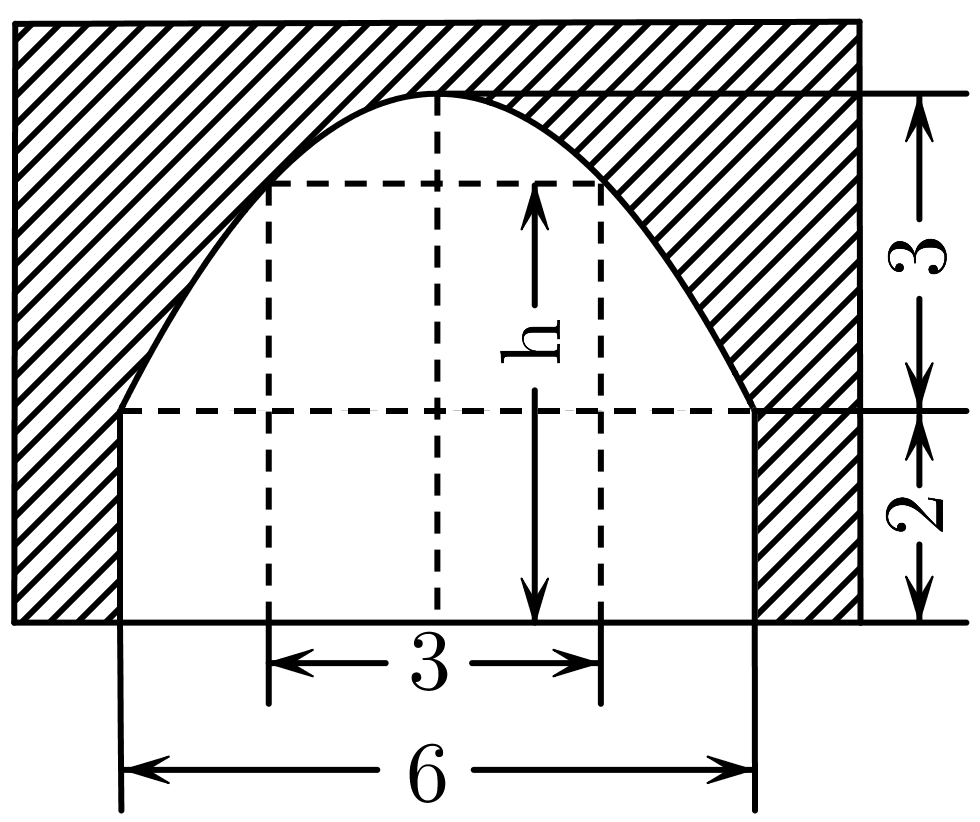
\includegraphics[width=40mm]{figs/15-16.png}}
\xiexwei{18mm}

{\ansblockgrayfalse
\begin{ansblock}[2章-练-课时15-16]
% ans:2章-练-课时15-16
\ansitem{23}{不能安全通过隧道。}
\ansnote{详解}{以抛物线顶点为原点、对称轴为\(y\)轴建系．由图：拱高3m、半宽3m，抛物线过\(A(3,-3)\)；矩形部分高2m、总高（顶点至地面）5m、地面\(y=-5\)．设\(x^{2}=-2py\)（\(p>0\)）：\(9=-2p\times (-3)\)，\(2p=3\)，方程\(x^{2}=-3y\)．\par\noindent 车居中：\(x=\pm 1.5\)处拱高\(y=-(1/3)\times 2.25=-0.75\)，净空\(=5-0.75=4.25\)(m)．\(4.25<4.5\)（车与集装箱总高），即使集装箱处于隧道正中，总高仍高于该处拱高，故不能安全通过．验算：\((\pm 1.5)^{2}=-3y\)得\(y=-0.75\)合；\(2p=3\)时准线\(y=3/4\)合．}
\end{ansblock}}

\liB{变式\textbf{24}}{中档(知识点三)}{}{早在一千多年之前，我国已经把溢流孔用于造桥技术，以减轻桥身重量和水流对桥身的冲击．现设桥拱上有4个溢流孔，桥拱和溢流孔的轮廓线均为抛物线的一部分，且4个溢流孔的轮廓线相同．根据图注尺寸，试分别求出这些抛物线的方程，及溢流孔与桥拱交点\(A\)，\(B\)，\(C\)的位置．（图注：桥拱所在抛物线过点(20,−5)，4个溢流孔轮廓线为全等抛物线，顶点分别为(−14,0)、(−7,0)、(7,0)、(14,0)，其中顶点(14,0)的溢流孔过点(20,−5)）}
\xiexwei{18mm}

{\ansblockgrayfalse
\begin{ansblock}[2章-拓-课时15-01]
% ans:2章-拓-课时15-01
{\parfillskip=0pt\rightskip=0pt plus 1fil\ansitem{24}{桥拱所在抛物线 y=−(1/80)x²；溢流孔所在抛物线分别为 y=−(5/36)(x+14)²、y=−(5/36)(x+7)²、y=−(5/36)(x−7)²、y=−(5/36)(x−14)²；交点 A((140/13),−(245/169))、B(10,−5/4)、C((70/13),−(245/676))。}}
\ansnote{详解}{设桥拱\(y=ax^{2}\)．由图注，桥拱过点\((20,-5)\)：\(-5=a\times 20^{2}\)，\(a=-1/80\)，桥拱\(y=-(1/80)x^{2}\)．①\par\noindent 设\(A\)所在溢流孔\(y=a_1(x-14)^{2}\)（顶点\((14,0)\)），亦过\((20,-5)\)：\(-5=a_1\times 36\)，\(a_1=-5/36\)．4孔轮廓相同、顶点\((\pm 7,0)\)、\((\pm 14,0)\)：\(y=-(5/36)(x\mp 7)^{2}\)、\(y=-(5/36)(x\mp 14)^{2}\)．②③\par\noindent 联立①②：\(400(x-14)^{2}=36x^{2}\)（两边乘2880），即\(91x^{2}-2800x+19600=0\)，\(\Delta=705600\)，\(\sqrt{\Delta}=840\)，\(x=20\)（\(y=-5\)）或\(x=140/13\)（\(y=-245/169\)），取交点\(A(140/13,-245/169)\)；联立①③：\(400(x-7)^{2}=36x^{2}\)，即\(91x^{2}-1400x+4900=0\)，\(\Delta=176400\)，\(\sqrt{\Delta}=420\)，\(x=10\)（\(y=-5/4\)）或\(x=70/13\)（\(y=-245/676\)），得\(C(70/13,-245/676)\)、\(B(10,-5/4)\)．验算：\(x=140/13\)：\(y=-(1/80)(140/13)^{2}=-19600/(80\times 169)=-245/169\)合；\(x=10\)：\(-100/80=-5/4\)合；\(x=70/13\)：\(-4900/(80\times 169)=-245/676\)合．}
\end{ansblock}}

\tjdnr{四}{实际应用与综合轨迹}{例\textbf{25}}{中档(知识点三)}{某城市在主干道统一安装了一种新型节能路灯，该路灯由灯柱和支架组成．支架\(ACB\)是抛物线\(y^{2}=2x\)的一部分，灯柱\(CD\)经过该抛物线的焦点\(F\)且与路面垂直，其中\(B\)为抛物线的顶点，\(DH\)表示道路路面，\(BF\parallel DH\)，\(A\)为锥形灯罩的顶，灯罩轴线与抛物线在\(A\)处的切线垂直．安装时，要求锥形灯罩的顶到灯柱所在直线的距离是1.5m，灯罩的轴线正好通过道路路面中的中线．(1)求灯罩轴线所在的直线方程；(2)若路宽为10m，求灯柱的高．}
\xiexwei{18mm}

{\ansblockgrayfalse
\begin{ansblock}[2章-拓-课时15-09]
% ans:2章-拓-课时15-09
\ansitem{25}{(1) y=−2x+6；(2) 6m。}
\ansnote{详解}{(1)\(|BF|=p/2=1/2\)，灯柱\(CD\)过焦点\(F(1/2,0)\)且\(A\)到灯柱距离1.5，得\(x_A=1/2+3/2=2\)；代入\(y^{2}=2x\)得\(y_A=2\)（取上半支），\(A(2,2)\)．设\(A\)处切线\(y-2=k(x-2)\)：与\(y^{2}=2x\)联立消\(x\)得\(ky^{2}-2y+4-4k=0\)，相切\(\Delta=4-4k(4-4k)=0\)，即\(16k^{2}-16k+4=0\)，\(k=1/2\)．灯罩轴线与切线垂直：斜率\(-2\)，方程\(y-2=-2(x-2)\)，即\(y=-2x+6\)．\par\noindent (2)路宽\(|DH|=10\)，灯罩轴线过路面中线，轴线与路面交点到\(y\)轴距离\(1/2+5=11/2\)．对\(y=-2x+6\)，\(x=11/2\)时\(y=-5\)，交点\((11/2,-5)\)，\(|FD|=5\)；又\(x=1/2\)代入\(y^{2}=2x\)得\(y=\pm 1\)，\(|CF|=1\)．灯柱高\(|CD|=|DF|+|FC|=6\)(m)．验算：\(16k^{2}-16k+4=4(2k-1)^{2}=0\)合；\(|CD|=6\)合．}
\end{ansblock}}

\liB{变式\textbf{26}}{中档(知识点三)}{\duoxuan\hspace{0.6em}}{已知正方体\(ABCD-A_1B_1C_1D_1\)的棱长为2，\(M\)为\(DD_1\)的中点，\(N\)为正方形\(ABCD\)所在平面内一动点，则下列命题正确的有\nobreak(\kongwei)}

\lxopt{A．若\(MN=2\)，则\(MN\)的中点的轨迹所围成图形的面积为\(\pi\)}

\lxopt{B．若\(N\)到直线\(BB_1\)与直线\(DC\)的距离相等，则\(N\)的轨迹为抛物线}

\lxopt{C．若\(D_1N\)与\(AB\)所成的角为\(\pi/3\)，则\(N\)的轨迹为双曲线}

\lxopt{D．若\(\angle ND_1B=\pi/6\)，则\(N\)的轨迹为椭圆}

{\ansblockgrayfalse
\begin{ansblock}[2章-拓-课时15-03]
% ans:2章-拓-课时15-03
\ansitem{26}{BCD}
\ansnote{详解}{A：\(D_1D\perp\)底面，\(DN=\sqrt{MN^{2}-MD^{2}}=\sqrt{4-1}=\sqrt{3}\)，\(N\)的轨迹是以\(D\)为圆心、\(\sqrt{3}\)为半径的圆．设\(MN\)中点\(P\)、\(MD\)中点\(Q\)，则\(PQ\parallel ND\)且\(PQ=\sqrt{3}/2\)，\(P\)的轨迹是以\(Q\)为圆心\(\sqrt{3}/2\)为半径的圆，面积\(\pi\times 3/4=3\pi/4\neq \pi\)，A错；\par\noindent B：\(N\)到\(B_1B\)的距离\(=NB\)（\(B_1B\perp\)底面），即\(N\)到定点\(B\)与定直线\(DC\)距离相等（\(B\)不在\(DC\)上），轨迹为抛物线，B对；\par\noindent C：\(AB\parallel D_1C_1\)，\(D_1N\)与\(D_1C_1\)所成角\(\pi/3\)，即\(D_1N\)为以\(D_1C_1\)为轴、轴截面顶角\(2\pi/3\)的圆锥母线，底面\(ABCD\)与轴\(D_1C_1\)平行，交线为双曲线，C对；\par\noindent D：\(D_1N\)为以\(D_1B\)为轴、顶角\(\pi/3\)的圆锥母线，平面\(ABCD\)与轴\(D_1B\)斜交，交线为椭圆，D对．故选BCD．}
\end{ansblock}}

\liB{变式\textbf{27}}{中档(知识点三)}{\duoxuan\hspace{0.6em}}{棱长为2的正方体\(ABCD-A_1B_1C_1D_1\)中，\(M\)，\(N\)分别为棱\(A_1D_1\)，\(AB\)中点，\(P\)为侧面\(BCC_1B_1\)一动点，下列说法正确的是\nobreak(\kongwei)}

\lxopt{A．异面直线\(AC\)与\(BM\)所成角的余弦值为\(\sqrt{2}/3\)}

\lxopt{B．若\(\triangle AC_1P\)的面积为\(\sqrt{3}\)，则动点\(P\)的轨迹为椭圆的一部分}

\lxopt{C．若点\(P\)到直线\(BC\)与直线\(C_1D_1\)的距离相等，则动点\(P\)的轨迹为抛物线的一部分}

\lxopt{D．过直线\(MN\)的平面\(\alpha\)与面\(ABCD\)所成角最小时，平面\(\alpha\)截正方体所得的截面面积为\(3\sqrt{3}\)}

{\ansblockgrayfalse
\begin{ansblock}[2章-拓-课时15-04]
% ans:2章-拓-课时15-04
\ansitem{27}{BCD}
\ansnote{详解}{以\(D\)为原点、\(DA\)、\(DC\)、\(DD_1\)为\(x\)、\(y\)、\(z\)轴建系：\(A(2,0,0)\)，\(C(0,2,0)\)，\(B(2,2,0)\)，\(M(1,0,2)\)．\par\noindent A：\(\overrightarrow{AC}=(-2,2,0)\)，\(\overrightarrow{BM}=(-1,-2,2)\)，\(|\cos\langle\overrightarrow{AC},\overrightarrow{BM}\rangle|=|\overrightarrow{AC}\cdot\overrightarrow{BM}|/(|\overrightarrow{AC}||\overrightarrow{BM}|)=|2-4+0|/(2\sqrt{2}\times 3)=\sqrt{2}/6\neq\sqrt{2}/3\)，A错；\par\noindent B：\(S=(1/2)|AC_1|\cdot h=\sqrt{3}\)，\(|AC_1|=2\sqrt{3}\)，得\(h=1\)：\(P\)在以\(AC_1\)为轴、半径1的圆柱面上，该圆柱面与侧面\(BCC_1B_1\)（与轴斜交）的交线为椭圆的一部分，B对；\par\noindent C：\(P\)在侧面\(BCC_1B_1\)上时，到\(C_1D_1\)的距离\(=|PC_1|\)，条件即\(|PC_1|\)等于\(P\)到直线\(BC\)的距离——到定点与定直线等距且\(C_1\)不在\(BC\)上，轨迹为抛物线的一部分，C对；\par\noindent D：取\(AD\)中点\(H\)，\(MH=2\)且\(MH\perp\)底面；当交线与\(AC\)平行（\(HN\perp AC\)）时二面角最小，截面为过\(M\)、\(N\)及四棱中点的正六边形，边长\(\sqrt{2}\)，面积\(6\times(\sqrt{3}/4)\times 2=3\sqrt{3}\)，D对．故选BCD．}
\end{ansblock}}

\tjdnr{四}{实际应用与综合轨迹}{例\textbf{28}}{中档(知识点三)}{在平面四边形\(ABCD\)中，满足\(AB=BC\)，\(CD=AD\)，且\(AB+AD=10\)，\(BD=8\)，沿着\(BD\)把\(\triangle ABD\)折起，使点\(A\)到达点\(P\)的位置，且使\(PC=2\)，则三棱锥\(P-BCD\)体积的最大值为\nobreak(\kongwei)}

\bindopt {\fontsize{10.5pt}{\qpTJgLeadLiti}\selectfont \makebox[\dimexpr0.5\linewidth-1em\relax][l]{A．12}\makebox[\dimexpr0.5\linewidth-1em\relax][l]{B．\(12\sqrt{2}\)}\par}
\bindopt {\fontsize{10.5pt}{\qpTJgLeadLiti}\selectfont \makebox[\dimexpr0.5\linewidth-1em\relax][l]{C．\(16\sqrt{2}/3\)}\makebox[\dimexpr0.5\linewidth-1em\relax][l]{D．\(16/3\)}\par}

{\ansblockgrayfalse
\begin{ansblock}[2章-拓-课时15-05]
% ans:2章-拓-课时15-05
\ansitem{28}{C}
\ansnote{详解}{折叠不变量：\(PB=AB\)，\(PD=AD\)，故\(PB+PD=10>BD=8\)，\(P\)在以\(B\)、\(D\)为焦点、长轴10、焦距8的椭圆上（不在长轴端点）．\par\noindent \(\triangle BPD\cong\triangle BCD\)（三边相等），得\(\angle PBD=\angle CBD\)．过\(P\)作\(PE\perp BD\)于\(E\)，连\(CE\)：\(\triangle BPE\cong\triangle BCE\)，得\(CE\perp BD\)且\(PE=CE\)，故\(BD\perp\)平面\(PCE\)．\(V_{P-BCD}=V_{B-PCE}+V_{D-PCE}=(1/3)S_{\triangle PCE}\cdot BD=(8/3)S_{\triangle PCE}\)．取\(PC\)中点\(F\)，\(EF\perp PC\)（\(PE=CE\)）：\(S_{\triangle PCE}=(1/2)\cdot PC\cdot EF=\sqrt{PE^{2}-1}\)（\(PC=2\)得\(CF=1\)）．\(PE\)的最大值为椭圆短半轴\(\sqrt{5^{2}-4^{2}}=3\)，故\(S_{\triangle PCE}\)最大\(=\sqrt{9-1}=2\sqrt{2}\)．\(V_{\max}=(8/3)\times 2\sqrt{2}=16\sqrt{2}/3\)，故选C．验算：\(EF=\sqrt{PE^{2}-CF^{2}}=\sqrt{PE^{2}-1}\)合；\(PE=3\)时\(EF=2\sqrt{2}\)，\(S=(1/2)\times 2\times 2\sqrt{2}=2\sqrt{2}\)合．}
\end{ansblock}}

\liB{变式\textbf{29}}{中档(知识点三)}{\duoxuan\hspace{0.6em}}{已知长方体\(ABCD-A_1B_1C_1D_1\)中，\(AB=BC=2\)，\(AA_1=2\sqrt{2}\)，点\(P\)是四边形\(A_1B_1C_1D_1\)内（包含边界）的一动点，设二面角\(P-AD-B\)的大小为\(\alpha\)，直线\(PB\)与平面\(ABCD\)所成的角为\(\beta\)，若\(\alpha=\beta\)，则\nobreak(\kongwei)}

\lxopt{A．点\(P\)的轨迹为一条抛物线}

\lxopt{B．线段\(PB\)长的最小值为3}

\lxopt{C．直线\(PA_1\)与直线\(CD\)所成角的最大值为\(\pi/4\)}

\lxopt{D．三棱锥\(P-A_1BC_1\)体积的最大值为\(2\sqrt{2}/3\)}

{\ansblockgrayfalse
\begin{ansblock}[2章-拓-课时15-06]
% ans:2章-拓-课时15-06
\ansitem{29}{BCD}
\ansnote{详解}{过\(P\)作\(PO\perp\)平面\(ABCD\)于\(O\)，\(OH\perp AD\)于\(H\)．\(AD\perp\)平面\(POH\)，故\(AD\perp PH\)，\(\angle PHO=\alpha\)；又\(\angle PBO=\beta\)，\(\alpha=\beta\)得\(OH=OB\)．\par\noindent \(O\)的轨迹：底面内到定点\(B\)与定直线\(AD\)等距的点集，即以\(B\)为焦点、\(AD\)为准线的抛物线在四边形\(ABCD\)内（含边界）的部分；\(P\)的轨迹为其上平移（以\(B_1\)为焦点、\(A_1D_1\)为准线），是抛物线的一部分而非整条，A错；\par\noindent B：\(|PB|^{2}=(2\sqrt{2})^{2}+|OB|^{2}\)，\(O\)为\(AB\)中点时\(|OB|_{\min}=1\)，故\(|PB|_{\min}=\sqrt{8+1}=3\)，B对；\par\noindent C：\(PA_1\)与\(CD\)所成角即\(OA\)与\(AB\)所成角\(\angle OAB\)．以\(AB\)中点\(M\)为原点建系，抛物线\(y^{2}=4x\)，\(A(-1,0)\)．设切线\(x=ty-1\)：代入得\(y^{2}-4ty+4=0\)，\(\Delta=16t^{2}-16=0\)，\(t=\pm 1\)，取\(t=1\)（\(O\)在四边形内），\(\angle OAB=\pi/4\)，最大值\(\pi/4\)，C对；\par\noindent D：\(V_{P-A_1BC_1}=V_{B-PA_1C_1}=(1/3)S_{\triangle PA_1C_1}\cdot BB_1\)，\(A_1C_1=2\sqrt{2}\)．\(P\)到\(A_1C_1\)距离最大\(\Leftrightarrow O\)到\(AC\)距离最大：\(O\)为\(AB\)中点时最大，值\((1/4)|BD|=\sqrt{2}/2\)．\(V_{\max}=(2\sqrt{2}/3)\times (1/2)\times 2\sqrt{2}\times (\sqrt{2}/2)=2\sqrt{2}/3\)，D对．故选BCD．验算：\(y^{2}=4x\)（焦点\(B(1,0)\)，准线\(x=-1\)即\(AD\)所在直线）：\(|OB|\)与\(|OH|\)分别为到焦点、准线的距离，等距即轨迹合；切线\(y=x+1\)过\(A(-1,0)\)，斜率1，\(\angle OAB=45^{\circ}\)合．}
\end{ansblock}}

\tjdnr{四}{实际应用与综合轨迹}{例\textbf{30}}{中档(知识点三)}{阿基米德（公元前287年～公元前212年）是古希腊伟大的物理学家，数学家和天文学家，并享有“数学之神”的称号．他研究抛物线的求积法，得出了著名的阿基米德定理．在该定理中，抛物线的弦与过弦的端点的两切线所围成的三角形被称为“阿基米德三角形”．若抛物线上任意两点\(A\)，\(B\)处的切线交于点\(P\)，则\(\triangle PAB\)为“阿基米德三角形”，且当线段\(AB\)经过抛物线的焦点\(F\)时，\(\triangle PAB\)具有以下特征：(1)\(P\)点必在抛物线的准线上；(2)\(PA\perp PB\)；(3)\(PF\perp AB\)．若经过抛物线\(y^{2}=8x\)的焦点的一条弦为\(AB\)，“阿基米德三角形”为\(\triangle PAB\)，且点\(P\)在直线\(x-y+6=0\)上，则直线\(AB\)的方程为\nobreak(\kongwei)}

\bindopt {\fontsize{10.5pt}{\qpTJgLeadLiti}\selectfont \makebox[\dimexpr0.5\linewidth-1em\relax][l]{A．\(x-y-2=0\)}\makebox[\dimexpr0.5\linewidth-1em\relax][l]{B．\(x-2y-2=0\)}\par}
\bindopt {\fontsize{10.5pt}{\qpTJgLeadLiti}\selectfont \makebox[\dimexpr0.5\linewidth-1em\relax][l]{C．\(x+y-2=0\)}\makebox[\dimexpr0.5\linewidth-1em\relax][l]{D．\(x+2y-2=0\)}\par}

\begin{ansblock}[2章-拓-课时15-02]
% ans:2章-拓-课时15-02
\ansitem{30}{A}
\ansnote{详解}{\(y^{2}=8x\)：\(p=4\)，准线\(x=-2\)，焦点\(F(2,0)\)．\(P\)在准线\(x=-2\)上，又在\(x-y+6=0\)上：\(P(-2,4)\)．\(k_{PF}=(0-4)/(2+2)=-1\)；由特征(3)\(PF\perp AB\)，得\(k_{AB}=1\)．\(AB\)过\(F(2,0)\)：\(y=x-2\)，即\(x-y-2=0\)，故选A．验算：\(P(-2,4)\)代入\(x-y+6=0\)：\(-2-4+6=0\)合．}
\end{ansblock}

\xiaojie{①识别：拱桥、隧道、路灯、门形建筑等实物轮廓建模与立体几何背景中轨迹判定的题，判归本题型；路径为“建系—设标准方程—代点定\(p\)—回实际量”.}
\bindp {\kaishu ②操作：以顶点为原点、对称轴为坐标轴建系使方程最简；印面无图的题按图注尺寸立式；立体几何轨迹用定义或圆锥曲线截线语义逐项判定.}
\bindp {\kaishu ③收束：应用题结论须带单位并回到题问（能否通过、位置坐标）；多选逐项给足判定理由，全对方可入选.}

% ---------- 探究点五 压轴：方程与存在性（印面 31） ----------
\tjdnr{五}{压轴：方程与存在性}{例\textbf{31}}{难(知识点三)}{已知抛物线\(y^{2}=2px\)（\(p>0\)）经过点\(P(4,4)\)，其焦点为\(F\)．(1)求抛物线\(C\)的方程；(2)设点\(Q\)在抛物线\(C\)上，试问在直线\(2x-y+6=0\)上是否存在点\(N\)，使得四边形\(PQFN\)是平行四边形？若存在，求出点\(Q\)的坐标；若不存在，说明理由．}
\xiexwei{18mm}

{\ansblockgrayfalse
\begin{ansblock}[2章-练-课时15-15]
% ans:2章-练-课时15-15
\ansitem{31}{(1) y²=4x；(2) 存在，此时 Q(9,6) 或 Q(4,−4)。}
\ansnote{详解}{(1)\(16=8p\)得\(p=2\)，\(C\)：\(y^{2}=4x\)．\par\noindent (2)\(F(1,0)\)．设\(N(t,2t+6)\)、\(Q(x_0,y_0)\)．四边形\(PQFN\)为平行四边形\(\Leftrightarrow\overrightarrow{PQ}=\overrightarrow{NF}\Leftrightarrow Q-P=F-N\)：\((4-t,-2t-2)=(x_0-1,y_0)\)，得\(x_0=5-t\)，\(y_0=-2t-2\)．\(Q\)在\(C\)上：\((-2t-2)^{2}=4(5-t)\)，即\(4t^{2}+8t+4=20-4t\)，\(t^{2}+3t-4=0\)，\(t=1\)或\(t=-4\)．\(t=1\)：\(N(1,8)\)，\(Q(4,-4)\)；\(t=-4\)：\(N(-4,-2)\)，\(Q(9,6)\)．\par\noindent 非退化核验（\(P\)、\(Q\)、\(F\)、\(N\)不共线，\(N\neq F\)）：\(t=1\)时\(\overrightarrow{PQ}=(0,-8)=\overrightarrow{NF}\)合；\(\overrightarrow{QF}=(-3,4)\)，\(\overrightarrow{PN}=\overrightarrow{P}-\overrightarrow{N}=(3,-4)\)，平行且相等合；四点不共线合，\(N(1,8)\neq F(1,0)\)合；\par\noindent \(t=-4\)时\(\overrightarrow{PQ}=(5,2)\)，\(\overrightarrow{NF}=\overrightarrow{F}-\overrightarrow{N}=(5,2)\)合；\(\overrightarrow{QF}=(-8,-6)\)，\(\overrightarrow{PN}=(8,6)\)合；斜率\(k_{PQ}=2/5\neq k_{QF}=3/4\)，四点不共线合，\(N\neq F\)合．两解均成立：存在\(N\)使\(PQFN\)为平行四边形，\(Q(9,6)\)或\(Q(4,-4)\)．验算：\(t^{2}+3t-4=(t-1)(t+4)\)合；\(Q(9,6)\)：\(36=4\times 9\)合；\(Q(4,-4)\)：\(16=16\)合．}
\end{ansblock}}

\xiaojie{①识别：首问求方程、次问存在性/平行四边形/通过性判定的两问压轴，判归本题型；基本路径为“求方程—设点表条件—解参数—核验作答”.}
\bindp {\kaishu ②操作：存在性题假设存在，列向量（或坐标）等式化为参数方程解之；平行四边形按顶点顺序用对边向量相等（\(\overrightarrow{PQ}=\overrightarrow{NF}\)）.}
\bindp {\kaishu ③收束：解出参数后须核验非退化（四点不共线、对角顶不重合）与题设范围，舍增根；应用判定题以不等量关系下结论.}

% ============================================================
% 课堂评价 G5（恒5＝3单选+2填空＝导槽 G1~G5；ketang 新制顺排可跨栏，禁 \vbox 装栏）
% 印面号 32—36
% ============================================================
\begin{ketang}{本组共5题（第32—36题），32—34为单选，35—36为填空．}

\jiancestem{{\fontsize{11.4pt}{14pt}\selectfont\heihao {\numboldjian 32}．}\hspace{4.1mm}\tieside{简单(知识点一)}\hspace{2.2mm}已知抛物线\(y^{2}=2px\)（\(p>0\)）上一点\(M\)到其准线及对称轴的距离分别为3和\(2\sqrt{2}\)，则\(p=\)\nobreak(\kongwei)}

\bindopt {\fontsize{10.5pt}{\qpTJgLeadPingjia}\selectfont \makebox[\dimexpr0.5\linewidth-1em\relax][l]{A．2}\makebox[\dimexpr0.5\linewidth-1em\relax][l]{B．2或4}\par}
\bindopt {\fontsize{10.5pt}{\qpTJgLeadPingjia}\selectfont \makebox[\dimexpr0.5\linewidth-1em\relax][l]{C．1或2}\makebox[\dimexpr0.5\linewidth-1em\relax][l]{D．1}\par}

{\ansblockgrayfalse
\begin{ansblock}[2章-导-课时15-G1]
% ans:2章-导-课时15-G1
\ansitem{32}{B}
\ansnote{详解}{设\(M(x_0,y_0)\)．到对称轴的距离\(|y_0|=2\sqrt{2}\)，故\(y_0^{2}=8\)；到准线\(x=-p/2\)的距离\(x_0+p/2=3\)，得\(x_0=3-p/2\)．代入\(y_0^{2}=2px_0\)：\(8=2p(3-p/2)=6p-p^{2}\)，即\(p^{2}-6p+8=0\)，解得\(p=2\)或\(p=4\)．两值均有\(x_0=3-p/2\geqslant 0\)（\(p=2\)时\(x_0=2\)；\(p=4\)时\(x_0=1\)），皆合题意，故选B．验算：\(p=2\)时准线\(x=-1\)，\(M(2,\pm 2\sqrt{2})\)，\(x_0+1=3\)合；\(p=4\)时准线\(x=-2\)，\(M(1,\pm 2\sqrt{2})\)，\(x_0+2=3\)合．}
\end{ansblock}}

\jiancestem{{\fontsize{11.4pt}{14pt}\selectfont\heihao {\numboldjian 33}．}\hspace{4.1mm}\tieside{简单(知识点二)}\hspace{2.2mm}抛物线\(y=-(1/8)x^{2}\)的准线方程是\nobreak(\kongwei)}

\bindopt {\fontsize{10.5pt}{\qpTJgLeadPingjia}\selectfont \makebox[\dimexpr0.5\linewidth-1em\relax][l]{A．\(x=1/32\)}\makebox[\dimexpr0.5\linewidth-1em\relax][l]{B．\(y=2\)}\par}
\bindopt {\fontsize{10.5pt}{\qpTJgLeadPingjia}\selectfont \makebox[\dimexpr0.5\linewidth-1em\relax][l]{C．\(y=1/32\)}\makebox[\dimexpr0.5\linewidth-1em\relax][l]{D．\(y=-2\)}\par}

\begin{ansblock}[2章-导-课时15-G2]
% ans:2章-导-课时15-G2
\ansitem{33}{B}
\ansnote{详解}{\(y=-(1/8)x^{2}\)即\(x^{2}=-8y\)，\(2p=8\)、\(p=4\)，开口向下，准线\(y=p/2=2\)，故选B．验算：焦点\((0,-2)\)、准线\(y=2\)，顶点\((0,0)\)到两者等距2合．}
\end{ansblock}

\jiancestem{{\fontsize{11.4pt}{14pt}\selectfont\heihao {\numboldjian 34}．}\hspace{4.1mm}\tieside{简单(知识点一)}\hspace{2.2mm}若动点\(M(x,y)\)满足\(5\sqrt{(x-1)^{2}+(y-2)^{2}}=|3x-4y+12|\)，则点\(M\)的轨迹是\nobreak(\kongwei)}

\bindopt {\fontsize{10.5pt}{\qpTJgLeadPingjia}\selectfont \makebox[\dimexpr0.5\linewidth-1em\relax][l]{A．圆}\makebox[\dimexpr0.5\linewidth-1em\relax][l]{B．椭圆}\par}
\bindopt {\fontsize{10.5pt}{\qpTJgLeadPingjia}\selectfont \makebox[\dimexpr0.5\linewidth-1em\relax][l]{C．双曲线}\makebox[\dimexpr0.5\linewidth-1em\relax][l]{D．抛物线}\par}

{\ansblockgrayfalse
\begin{ansblock}[2章-导-课时15-G3]
% ans:2章-导-课时15-G3
\ansitem{34}{D}
\ansnote{详解}{两边同除以5：\(\sqrt{(x-1)^{2}+(y-2)^{2}}=|3x-4y+12|/5\)，而\(|3x-4y+12|/\sqrt{3^{2}+4^{2}}\)恰为\(M\)到直线\(3x-4y+12=0\)的距离．故动点\(M\)到定点\((1,2)\)的距离等于它到定直线\(3x-4y+12=0\)的距离；又\(3\times 1-4\times 2+12=7\neq 0\)，定点不在定直线上，由抛物线的定义，轨迹是以\((1,2)\)为焦点、\(3x-4y+12=0\)为准线的抛物线，故选D．说明：系数5的作用仅是把右端配成点到直线距离的标准形式（\(5=\sqrt{3^{2}+(-4)^{2}}\)），并非离心率记号．}
\end{ansblock}}

\jiancestem{{\fontsize{11.4pt}{14pt}\selectfont\heihao {\numboldjian 35}．}\hspace{4.1mm}\tieside{简单(知识点二)}\hspace{2.2mm}已知抛物线的顶点在原点，对称轴为坐标轴，焦点在直线\(x-2y-4=0\)上，求抛物线的方程．}
\xiexwei{7mm}

{\ansblockgrayfalse
\begin{ansblock}[2章-导-课时15-G4]
% ans:2章-导-课时15-G4
\ansitem{35}{y²=16x 或 x²=−8y}
\ansnote{详解}{直线\(x-2y-4=0\)与坐标轴的交点：令\(y=0\)得\(A(4,0)\)；令\(x=0\)得\(B(0,-2)\)．①焦点为\(A(4,0)\)：开口向右，设\(y^{2}=2px\)（\(p>0\)），\(p/2=4\)得\(p=8\)，方程\(y^{2}=16x\)；②焦点为\(B(0,-2)\)：开口向下，设\(x^{2}=-2py\)（\(p>0\)），\(p/2=2\)得\(p=4\)，方程\(x^{2}=-8y\)．综上，所求抛物线的方程为\(y^{2}=16x\)或\(x^{2}=-8y\)．验算：\(y^{2}=16x\)的焦点\((4,0)\)满足\(4-0-4=0\)，在直线上合；\(x^{2}=-8y\)的焦点\((0,-2)\)满足\(0+4-4=0\)，在直线上合．}
\end{ansblock}}

\jiancestem{{\fontsize{11.4pt}{14pt}\selectfont\heihao {\numboldjian 36}．}\hspace{4.1mm}\tieside{简单(知识点二)}\hspace{2.2mm}已知抛物线的焦点在\(x\)轴上，抛物线上的点\(M(-3,m)\)到焦点的距离等于5，求抛物线的标准方程和\(m\)的值．}
\xiexwei{7mm}

\begin{ansblock}[2章-导-课时15-G5]
% ans:2章-导-课时15-G5
\ansitem{36}{y²=−8x；m=±2√6}
\ansnote{详解}{\(M(-3,m)\)的横坐标为负，抛物线开口向左，设\(y^{2}=-2px\)（\(p>0\)），则焦点\(F(-p/2,0)\)，准线\(x=p/2\)．由抛物线的定义，\(|MF|\)等于\(M\)到准线的距离：\(p/2+3=5\)，得\(p=4\)，故标准方程为\(y^{2}=-8x\)．将\(M(-3,m)\)代入：\(m^{2}=24\)，\(m=\pm 2\sqrt{6}\)．验算：焦点\(F(-2,0)\)：\(|MF|=\sqrt{(-3+2)^{2}+m^{2}}=\sqrt{1+24}=5\)合（两点距与定义两法互证）．}
\end{ansblock}

\end{ketang}

% ---- 尾块（\tailfill 置 \end{multicols} 前；无参＝内容尾随框，件侧不擅自定高） ----
\tailfill

\end{multicols}

\end{document}

